
\subsection{Solución iterativa}

La solución iterativa a este problema es simple, se recorre la colección de puntos y por cada punto se le compara contra todos los demás calculando la distancia como $ \sqrt{ (x_{i}-x_{j})^{2} +(y_{i}-y_{j})^{2}} $, cada vez que una distancia sea inferior al mínimo anterior actualizamos cuales son los puntos más cercanos. Cuando ya comparamos todos los puntos contra todos el resultado es el par de puntos cuya distancia es seguro es mínima.

Es evidente que esta solución tanto en peor como en el mejor de los casos compara todos los puntos contra todos por lo que podemos decir que la complejidad de este algoritmo es O($n^{2}$) siendo {\em n} la cantidad de puntos en el plano. Por lo que solo es recomendable usar esta variante en problemas de concursos cuando la cantidad de puntos no superen los 1000.

\subsection{Divide y Conquista}

\begin{itemize}
	\item {\bf Dividir:} Partimos que tenemos los puntos almacenados en alguna estructura de dato secuencial. Si son pocos puntos podemos aplicar la primera variante. Si hay más puntos de lo permisible entonces trazamos una línea vertical {\em l} que subdivide a la colección P de puntos en dos colecciones aproximadamente del mismo tamaño, {\em Pl} y {\em Pr}. 
	\item {\bf Conquistar:} Recursivamente aplicamos el procedimiento en ambas colecciones por lo que obtenemos $\delta_{l}$ y $\delta{r}$ distancias mínimas
	para ambas colecciones. De ambas obtenemos $\delta=min(\delta_{l}, \delta{r})$.
	\item {\bf Combinar:} Lamentablemente $\delta$ no es el resultado final, ya que se podría darse la línea {\em l} que hemos elegido pasa justo entre dos puntos que están a distancia mínima. Debemos chequear si no hay dos puntos que están a distancia mínima. Debemos chequear si no hay dos puntos, uno a cada lado de la línea, cuya distancia sea menor que $ \delta $. En primer lugar observemos que no necesitamos chequear todos los puntos, si un punto esta a mayor distancia de {\em l} que $\delta$ entonces es seguro no hay vecino del otro lado de la línea que pueda formar una distancia menor que $\delta$. Creamos una lista  $P_{k}$ de puntos que están a menos de $\delta$ de cada lado de {\em l}. Determinamos entonces la distancia mínima para los puntos de $P_{k}$ que llamaremos $\delta'$ y devolvemos la distancia sino los dos puntos que están a dicha distancia uno del otro. 
\end{itemize}

El problema consiste en analizar cómo encontrar la distancia mínima en $P_{k}$, lo cual requiere un poco de astucia. Para optimizar el algoritmo queremos encontrar la distancia mínima en $P_{k}$ en tiempo O(n) vamos demostrar que esto puede hacerse suponiendo que los puntos de $P_{k}$ están ordenados por la coordenada {\em y}, luego tendremos que resolver como ordenar los puntos.

\begin{figure}[h]
	\centering 
	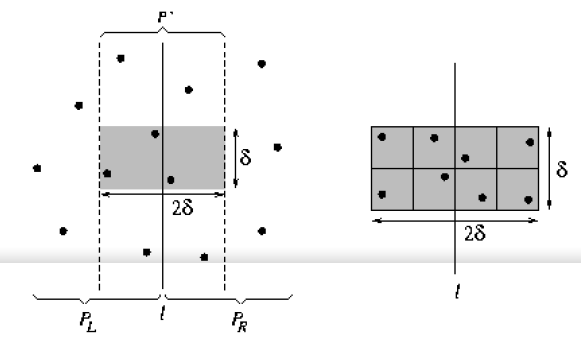
\includegraphics[scale=0.6]{img/closest_pair_1}
	\label{contexto:figura5}
\end{figure}

Supongamos que los puntos de $P_{k}$ están ordenados de acuerdo a su coordenada {\em y}. Consideremos un punto $P_{k}$[i] en lista ordenada. Cuál es el punto más cercano a $P_{k}$[i]. Podemos restringir la búsqueda a los puntos que tienen índice {\em j} mayor que {\em i} ya que el proceso lo vamos a hacer para todos los puntos (si el vecino más cercano está arriba, entonces esto ya fue analizado cuando buscamos el vecino de dicho punto). Podríamos pensar que necesariamente el vecino más cercano es  $P_{k}$[i+1], pero esto no es verdad, dos puntos que tienen distancia mínima en cuanto a la coordenada y no necesariamente tienen distancia mínima en el plano, queremos saber que tan lejos tenemos que buscar hasta $P_{k}$[i+2]?, $P_{k}$[i+8]? tal vez podamos acotar la búsqueda a una cantidad constante de puntos.

Resulta que podemos limitar la cantidad de puntos a buscar y además resulta que no nos hace falta analizar más de 7 puntos en la lista $P_{k}$ para cada punto.

Resumiendo el funcionamiento del algoritmo:

\begin{itemize}
	\item {\bf Presort:} Dada la lista {\em P}, hacemos dos copias {\em PX} y {\em PY}. Ordenamos {\em PX} por la coordenada {\em x} y la lista {\em PY} por las coordenadas {\em y}.
	\item {\bf Parte Recursiva:} DistMin(X,Y)
	\begin{itemize}
		\item {bf Condición de corte:} Si la cantidad de puntos es menor que 4 entonces resolvemos el problema por fuerza bruta y devolvernos la distancia mínima $\delta$ analizando todas las distancias posibles.
		\item {\bf Dividir:} Sino, sea {\em l} la mediana de las coordenadas {\em x} de {\em PX}. Dividimos ambas listas {\em PX} y {\em PY} por esa línea, manteniendo el orden, creando {\em X$_{l}$, X$_{r}$, Y$_{l}$, Y$_{r}$ }.
		\item {\bf Conquistar:} $\delta_{l}=DistMin(X_{l},Y_{l})$ , $\delta_{r}=DistMin(X_{r},Y_{r})$.
		\item {\bf Combinar:} $\delta=min(\delta_{l}, \delta{r})$ . Creamos la lista $Y_l$ copiando 
		todos los puntos de {\em Y} que están a distancia menor que $\delta$ de {\em l}. Para {\em i} 
		desde 1 hasta la longitud de $Y_l$ y para {\em j} desde {\em i+1} hasta {\em i+7} calcular 
		la distancia entre $Y_l$[i] y $Y_l$[j]. Sea $\delta'$ la distancia mínima entre dichas 
		distancias. Devolver min($\delta$, $\delta'$).
	\end{itemize}
\end{itemize}

\subsection{Línea de barrido}

Barreremos el plano de izquierda a derecha (o de derecha a izquierda es una posibilidad) y cuándo se alcance alcance un punto computaremos todos los puntos candidatos cercanos a este (los candidatos que puede estar en el par más cercano).

Por lo que haremos las siguientes operaciones:
\begin{enumerate}
	\item Ordenamos los puntos de izquierda a derecha por el eje {\em x}.
	\item Por cada punto:
	\begin{enumerate}
		\item Quitamos de los candidatos todo el punto que está más allá en el eje {\em x}  de la distancia mínima actual.
		\item Tomamos a todos los candidatos que son localizados a igual o menor distancia que la distancia mínima del punto actual en eje vertical.
		\item Probamos para la distancia mínima todos los candidatos encontrados con el punto actual.
		\item Y finalmente le añadimos el punto actual a la lista de candidatos.
	\end{enumerate}
\end{enumerate}

Así es que cuando encontramos una distancia mínima nueva , podemos hacer más pequeños el rectángulo de candidatos en el eje de las abscisas y más pequeño en el eje vertical. Así hacemos mucho menos comparaciones entre los puntos.